\documentclass{book}

\usepackage[reqno]{amsmath} % Paquete para el manejo de expresiones matemáticas [reqno], [leqno] y [fleqn]
\usepackage{amsthm}
\usepackage{amssymb,amsmath,latexsym} %Paquete para llamar símbolos matemáticos
\usepackage{tabularx,booktabs,ragged2e}
\usepackage{amsfonts}
\usepackage[mathscr]{euscript}
\usepackage{graphicx} %paquete para el manejo de transformaciones geométricas de imagénes
\usepackage{color} %paquete para el manejo de color en textos.
%\usepackage[utf8]{inputenc} %paquete para el manejo de caracteres acentuados
\usepackage[french,spanish]{babel} %paquete que genera documentos en diferentes idiomas
\usepackage{enumerate}
\usepackage{multicol} % Paquete para modificar el número de columnas
\usepackage{layout} % Paquete  para revisar los valores de 
\usepackage{verbatim}
\usepackage[all]{xy} 
\usepackage{pgfplots}
%graficos
\usepackage{pgfplots}
\pgfplotsset{compat=1.15}
\usepackage{mathrsfs}
\usetikzlibrary{arrows}
\pagestyle{empty}
%graficos
\pagestyle{myheadings}  % Estilo de página
%\pagenumbering{arabic} % Estilo de numéración
\hoffset1cm
\newcounter{Teorema}
\newcommand{\Teorema}{\stepcounter{Teorema}{\bf Teorema \theTeorema.} }
\DeclareMathOperator{\arcsec}{arcsec} % Creación de nuevos comandos en latex
\DeclareMathOperator{\Var}{Var}
\DeclareMathOperator*{\Hom}{Hom}
\setcounter{MaxMatrixCols}{15}
\allowdisplaybreaks % Control de cambios de página en alineaciones
\decimalpoint
%\renewcommand{\theequation}{\thesection.\arabic{equation}}
\numberwithin{equation}{section}
%\renewcommand{\theequation}{\theparentequation\arabic{equation}}
%% Nuevos teoremas
\theoremstyle{plain}  % Requiere el paquete amsthm
\newtheorem{thm}{Teorema}[section]
\newtheorem*{Dem}{Demostración}
\newtheorem{Corol}[thm]{Colorario}
\newtheorem{Prop}[thm]{Proposición}
\newtheorem{axiom[thm]}{Axioma}
\newtheorem{conj}{Conjetura}
\newtheorem{Def}{Definición}[section]
\newtheorem{Ej}{Ejemplo}[section]
\newtheorem{notacion}[Def]{Notación}
\newtheorem{nota}[Def]{Nota}
\renewcommand{\qedsymbol}{$\heartsuit$}
\providecommand{\abs}[1]{\lvert#1\rvert} %valor absoluto
\providecommand{\norm}[1]{\lVert#1\rVert} %norma
\usepackage{fancyhdr}
\pagestyle{empty}
\usepackage{pgfplots}
\usepackage{mathrsfs}
\usepackage{tcolorbox}
\usepackage{amsmath, amsthm, amssymb}
\usepackage{mathrsfs}
\usepackage{graphicx}
\usepackage{geometry}
\usepackage{amsmath}
\spanishdecimal{.}
\usepackage{color}
\usepackage{multicol}
\usepackage{bbding}
\usepackage{stackrel}
\usepackage{hyperref}
\usepackage{geometry}
\usepackage{multicol}
\usepackage{amsfonts}
\usepackage{multicol}
\usepackage{bbding}
%\usepackage[manejador]{color,graphicx}

%colores 
\definecolor{dorado}{cmyk}{0,0.10,0.84,0}
\definecolor{melon}{cmyk}{0,0.29,0.84,0}
\definecolor{naranja}{cmyk}{0,0.42,1,0}
\definecolor{durazno}{cmyk}{0,0.46,0.50,0}
\definecolor{fresa}{cmyk}{0,1,0.50,0}
\definecolor{ladrillo}{cmyk}{0,0.77,0.87,0}
\definecolor{violeta}{cmyk}{0.07,0.90,0,0.34}
\definecolor{purpura}{cmyk}{0.45,0.86,0,0}
\definecolor{aguamarina}{cmyk}{0.85,0,0.33,0}
\definecolor{esmeralda}{cmyk}{0.91,0,0.88,0.12}
\definecolor{pino}{cmyk}{0.92,0,0.59,0.25}
\definecolor{oliva}{cmyk}{0.64,0,0.95,0.40}
\definecolor{canela}{cmyk}{0.14,0.42,0.56,0}
\definecolor{cafe}{cmyk}{0,0.81,1,0.60}
\definecolor{marron}{cmyk}{0,0.72,1,0.45}
\definecolor{gris-claro}{cmyk}{0,0,0,0.30}
\definecolor{gris-oscuro}{cmyk}{0,0,0,0.50}

\begin{document}
    \chapter*{Ejercicios en parejas Corte 1}
    \noindent
    Wilson Eduardo Jerez Hernández, 20181167034 \\
    El Juliancho parancho
    \section*{Ejercicios 1.1}
    \subsection*{21} 
    Un estanque inicialmente contiene 1,000,000 galones de agua y una cantidad desconocida de un químico indeseable. 
    El agua que contiene 0.01 g de este químico por galón fluye hacia el estanque a razón de 300 gal/h. 
    La mezcla sale a la misma velocidad, por lo que la cantidad de agua en el estanque permanece constante. 
    Suponga que el producto químico se distribuye uniformemente por todo el estanque. 
    \begin{itemize}
        \item[(a)]Escriba una ecuación diferencial para la cantidad de sustancia química en el estanque en cualquier momento
        \item[(b)] ¿Qué cantidad de producto químico habrá en el estanque después de un largo tiempo?
    \end{itemize}
    \subsection*{27}
    En cada uno de los problemas 26 a 33, dibuje un campo direccional para la ecuación diferencial dada. Con base en el campo de dirección, determine el comportamiento de y cuando
    $t \to \infty$. Si este comportamiento depende del valor inicial de $y$ en $t = 0$, describa esta dependencia. Tenga en cuenta que los lados derechos de estas ecuaciones dependen tanto de $t$ como de $y$; por lo tanto, sus soluciones pueden exhibir un comportamiento más complicado que las del texto.
    \\ 
    \begin{itemize}
        \item[*] $y'=te^{-2t}-2y$
    \end{itemize}
    \section*{Ejercicios 1.3}
    \subsection*{14}
    En cada uno de los problemas del 7 al 14, verifique que cada función dada sea una solución de la ecuación diferencial.
    \begin{itemize}
        \item[*] $y'-2ty=1$; $y=e^{t^{2}}\int_{0}^{t}e^{-s^{2}}ds+e^{t^{2}}$
    \end{itemize}
    \subsection*{30}
    \subsection*{Preliminares} 
    Un problema físico simple que conduce a una ecuación diferencial no lineal 
    es el péndulo oscilante. El ángulo $\theta$ que forma un péndulo oscilante de longitud L con 
    la dirección vertical (ver Figura 1) satisface la ecuación:
    \begin{equation}
        \frac{d^{2}\theta}{dt^{2}} + \frac{g}{L} \sin{\theta} = 0
    \end{equation}
    \begin{figure}[h]
        \centering
        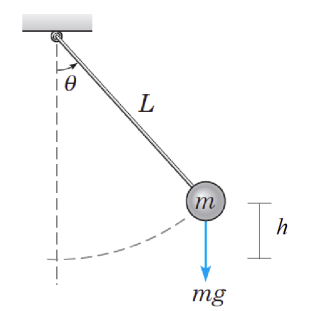
\includegraphics[width=0.4\linewidth]{imagenes/EDC1.png}
        \caption{Un péndulo oscilante.}
      \end{figure} \\
    Otra forma de derivar la ecuación del péndulo (0.0.1) se basa en el principio de conservación de la energía
    \begin{itemize}
        \item[(a)] Demuestre que la energía cinética T del péndulo en movimiento es
        \begin{equation*}
            T=\frac{1}{2}mL^{2}(\frac{d\theta}{dt})^{2}
        \end{equation*}
        \item[(b)] Demuestre que la energía potencial V del péndulo, relativa a su posición de reposo, es
        \begin{equation*}
            V = mgL(1-\cos{\theta})
        \end{equation*} 
        \item[(c)] Por el principio de conservación de la energía, la energía total $E = T + V$ es constante. 
        Calcule $dE/dt$, iguale a cero y demuestre que la ecuación resultante se reduce a la Eq. (0.0.1).
    \end{itemize}
\end{document}